\documentclass{article}
\newcommand{\exptitle}{Stirling's Engine}
\newcommand{\course}{PHYS3113 - Thermodynamics and Statistical Mechanics}

\usepackage{graphicx}
\usepackage{pgf}
\usepackage{lmodern}
\usepackage{import}
\usepackage{booktabs}
\usepackage{tabu}
\usepackage{float}
\usepackage[hidelinks]{hyperref}
\usepackage{amsmath}
\usepackage{amsfonts}
\usepackage[margin=1in]{geometry}
\usepackage{pythonhighlight}
\usepackage[toc]{appendix}
\usepackage{float}
\usepackage{placeins}
\usepackage{natbib}
\usepackage{lmodern}
\usepackage{subfig}
\usepackage[utf8]{inputenc}
\usepackage[T1]{fontenc}
\usepackage{upgreek}
\usepackage{chemmacros}
\usepackage{braket}
\usepackage{newpxtext,newpxmath}
\usepackage{tikz}

\DeclareMathOperator{\sech}{sech}
\DeclareMathOperator{\cosech}{cosech}

\setlength{\parskip}{1em}
\setlength{\parindent}{0em}

\begin{document}

\begin{titlepage}
    \begin{center}
        \vspace*{7cm}

        \Huge
        \textbf{\exptitle}

        \vspace{0.5cm}
        \LARGE
        \course

        \vspace{1.5cm}

        \textbf{Toby Nguyen - z5416116}
    \end{center}
\end{titlepage}

\tableofcontents


\section{Introduction}
The Stirling Engine is a heat engine that uses a fluid such as air or other gas 
to produce mechanical work. By exposing the fluid to different temperatures, the 
fluid will expand and contract, producing that mechanical work, effectively 
converting heat energy to mechanical work. The thermodynamic cycle can be found 
in the Theoretical pre work below.

Stirling Engines can also be used as a refrigerator by reversing the thermodynamic 
cycle. This allows it for a wide range of applications such as engine-powered aircraft 
or autmotive engines as well as solar power generation and cryocooling.

\section{Method}
\subsection{Measuring Mechanical Power}
\subsubsection{Theory}
From classical mechanics, the mechanical power of a rotating object is given 
by 

\begin{equation}
    P = \tau \omega.
\end{equation}

Since, the torque of the object is dependent on the angular velocity of the 
object we have to account for this dependence,

\begin{equation}
    P = \tau (\omega) \omega.
\end{equation}

Then we find that the mechanical power of a system has quadratic dependence on 
its angular velocity and so we can model the mechanical power of the system 
based on the following relationship,

\begin{equation}
    P = a\omega^2 + b\omega + c 
\end{equation}

where $a,\: b,\: c$ are fitted parameters.

\subsubsection{Experiment setup}
A torque meter was attached to the rotating axle of the Stirling Engine and 
the counter weight would rotate the needle to measure the applied torque of 
the engine. The smallest increments on the torque reading was $1 \times 10^{-3}
\text{ Nm}^{-1}$, leading to an absolute uncertainty of $\pm 0.5 \times 10^{-3}
\text{ Nm}^{-1}$. The major source of uncertainty for this experiment and for 
all other experiments was the frequency reading. This is because the frequency 
of the spinning wheel was dependent on the temperature of the engine which was 
constantly flunctuating. To obtain an uncertainty value, we can use the percentage 
uncertainty from the temperature readings. Since there are two temperature readings,
we will take a percentage uncertainty of both temperature measurements and then 
add them in quadrature.

From the table in Figure \ref{tab:table1}, we calculate the standard deviation 
and average of $T_h$ and $T_c$. Taking the quotient of the two values and then 
summing them in quadrature gives us an percentage uncertainty of 15.7\%. The 
percentage uncertainty in the torque meter readings was found by taking the 
average of the quotient of 0.5 and the torque readings which came out to be 
5.2\%.

\subsection{Measuring Electrical Power}
\subsubsection{Theory}
The torque done by the Stirling Engine is used to spin the coil of a generator.
The electromotive force ($emf$) produced by the generator is given by Faraday's 
law,

\begin{equation}
    emf = -n\frac{\Delta \Phi}{\Delta t}.
\end{equation}

As the magnetic flux is a function of angular displacement, we can say that the 
$emf$ is a function of angular velocity. The power produced in the circuit is 
given by

\begin{align}
    P &= V(\omega)I \\
    &= \frac{V(\omega)^2}{R}. 
\end{align}

Again, we note the quadratic dependence of angular velocity and so we can model 
electrical power as a function of angular velocity as a quadratic,

\begin{equation}
    P = a\omega^2 + b\omega + c 
\end{equation}

where $a,\: b,\: c$ are fitted parameters.

\subsubsection{Experimental setup}
The torque meter and needle and mass apparatus were detached from the engine. A 
elastic rubber band was placed along the circumference of the Stirling Engine wheel 
and connected to a large pulley. The pulley would then spin a coil in a magnetic 
field to induce an emf. The circuit is set up as shown in Figure \ref{fig:circuit}. 

\begin{figure}[H]
    \centering
    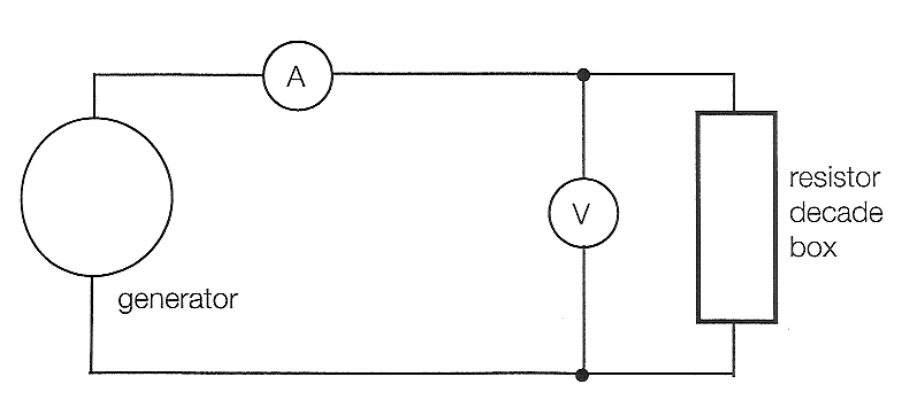
\includegraphics[width=0.7\textwidth]{../Figures/circuitdiagram.png}
    \caption{Circuit diagram displaying the circuit used in the electrical power 
    experiment.}
    \label{fig:circuit}    
\end{figure}

The induced emf would give rise to a current in the circuit. Increasing the electrical 
load by increasing resistance in the decade box would decrease the current in the 
coil which would lower the emf produced, allowing for the Stirling Engine to spin 
faster. Conversely, decreasing the load would increase the current in the circuit, 
increasing the emf induced which then increases the opposition to the torque produced 
by the Stirling Engine.

The major source of uncertainty in this experiment, like the one previous, would 
be the temperature and frequency readings. The method of uncertainty calculation was 
repeated for this experiment, achieving a value of 8.9\% .This experiment introduces two new 
sources of uncertainty being the ammeter and voltmeter readings. According to the 
Sanwa multimeter manual, the voltmeter has an accuracy of $\pm0.9\%rdg + 2dgt$ and 
the ammeter has an accuracy of $\pm1.8 \%rdg + 6dgt$ in their respective ranges.
The decade box used as the resistance load has an uncertainty of $\pm 1\%$. A lengthy 
script doing these calculations can be found in the Appendix, nevertheless we obtain 
an uncertainty of 8.7\%, mainly due to major contributions from the voltmeter readings.

\subsection{Cooling}
\subsubsection{Theory}
After shutdown, both chambers of the engine will cool and the relationship 
between the temperature of the system over time can be modelled using Newton's
Law of Cooling.

\begin{equation}
    \frac{dT_h}{dt} = -k(T_h - T_c).
\end{equation}

Since the temperature function of the two chambers are simply exponentials, we 
can take the temperature difference and model it over time.

\begin{equation}
    T_{\text{diff}}(t) = T_{\text{ambient}} + (T_0 - T_{\text{ambient}})e^{-kt}.
\end{equation}

\subsubsection{Experimental setup}
The ammeter, voltmeter and the decade box was disconnected. The flame was removed 
and the engine was allowed to cool. The uncertainty in this experiment was calculated 
by using the temperature uncertainty values found in the mechanical power experiment.

\section{Results}
\begin{figure}[H]
    \centering
    \scalebox{0.75}{\input{../Figures/mechpower.pgf}}
    \caption{Scatter plot displaying the results of increasing the applied 
    counter torque on the engine over the range of 0 to 20 $\times 10^{-3} \:  
    \text{Nm}^{-1}$.}
    \label{fig:mechpower}
\end{figure}
\begin{figure}[H]
    \centering
    \scalebox{0.75}{\input{../Figures/elecpower.pgf}}
    \caption{Scatter plot displaying the results of decreasing resistance 
    in the load in the range of magnitudes from $10^7$ to $1$.}
    \label{fig:elecpower}
\end{figure}

\begin{figure}[H]
    \centering
    \scalebox{0.75}{\input{../Figures/combined.pgf}}
    \caption{Plot comparing the peaks and shape of the two parabolas}
    \label{fig:combined}
\end{figure}

\begin{figure}[H]
    \centering
    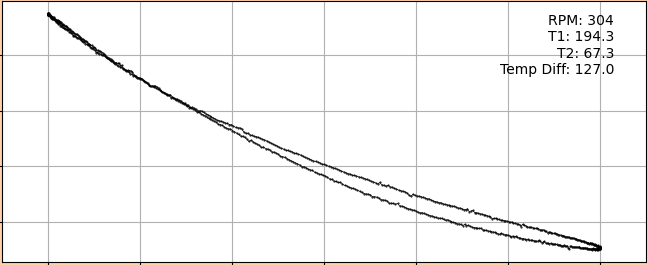
\includegraphics[width=0.4\textwidth]{../Figures/2 ohms.PNG}
    \hspace{0.5cm}
    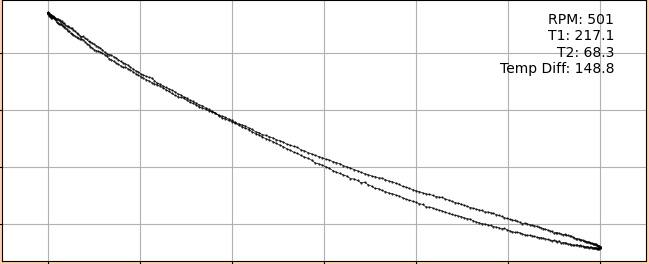
\includegraphics[width=0.4\textwidth]{../Figures/30 ohms.PNG}
    \vspace{0.5cm}
    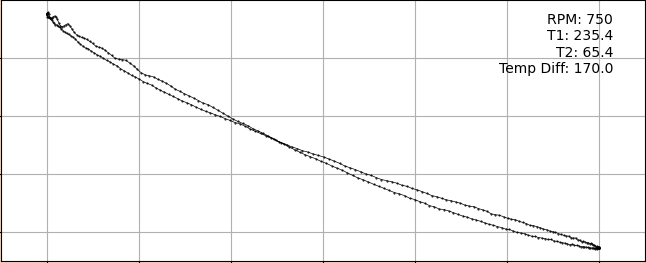
\includegraphics[width=0.4\textwidth]{../Figures/11111110 ohms.PNG}
    \hspace{0.5cm}
    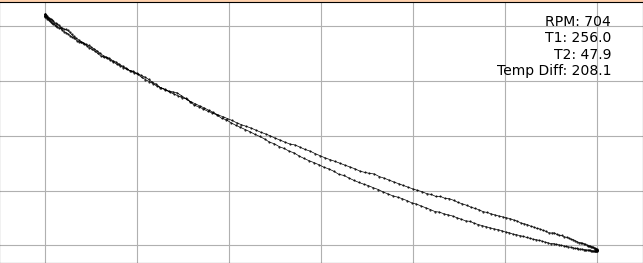
\includegraphics[width=0.4\textwidth]{../Figures/12 Nm.PNG}
    \caption{PV diagrams of (a) Top left the engine as a generator 
    providing current to a circuit with a load of 2 $\Omega$ (b) Same
    as befeore but with 30 $\Omega$ (c) Max resistance of 11111110 $\Omega$
    (d) The engine providing mechanical power against a counter torque of 
    $12 \times 10^{-3} \text{ Nm}^{-1}$.}
    \label{fig:PVdiagrams}
\end{figure}

\begin{figure}[H]
    \centering
    \scalebox{0.75}{\input{../Figures/cooling.pgf}}
    \caption{Exponential decay of temperature difference between the 
    two chambers.}
    \label{fig:cooling}
\end{figure}

\section{Analysis}
\subsection{Optimal angular velocity}
Comparing the two parabolas produced by different types of loads in Figure 
\ref{fig:combined}, we can see that the optimal angular velocity is substantially 
different between the two. We find that for the mechanical load experiment, the 
optimal angular velocity was found to be $45.7 \pm 7$ rads$^{-1}$ and for the 
electrical load experiment, the optimal angular velocity was found to be $56.4 
\pm 5$ rads$^{-1}$. We can also compare the peaks of the two parabolas, using 
the formula 

\begin{equation}
    \omega_{peak} = -\frac{b}{2a}.
\end{equation}

The experimental peak as derived from the parabola of best fit for the mechanical 
load is $60.6$ and for the electrical load, the optimal angular velocity is predicted 
to be $47.5$. We find that neither peak value agree with the predicted value for the 
same experiment.

\subsection{Work done by system}
By finding the areas found in the PV diagrams in Figure \ref{fig:PVdiagrams}, we can 
calculate the work done by the system per cycle. One rectangle in the grid weighs $0.0941$ g.
The half rectangle on the bottom part of the diagrams weighs $0.0468$ g. For the 
PV diagram with a load of $2 \: \Omega$, the percentage of the average area of the curve compared 
to the weight of the paper is then,

\begin{align}
    S &= \frac{0.1003+0.0599}{2\times(18\times0.0941+6\times0.0468)} \\
    &= 0.041 \text{ (mV)}^2
\end{align}

To convert this reading into a work done per cycle reading we use the conversion factors, $V_{\text{factor}}
= 417 \text{ mV/mL}$ and $P_{\text{factor}} = 3.75 \times 10^{-5} \text{ V/Pa}$. Therefore, the work done per 
cycle is then 

\begin{align}
    W_{\text{per cycle}} &= S \times V_{\text{factor}} \times P_{\text{factor}} \\
    &= 0.041 \times 417 \times 3.75 \times 10^{-5} \\
    &= 6.4 \times 10^{-4} \text{ J/cycle}
\end{align}

To convert this into a power reading, we can multiple by frequency, so for the $2 \Omega$ load, the power 
produced by the engine is 

\begin{align}
    P_{2\Omega} &= 6.4 \times 10^{-4} \times 5.06 \\
    &= 3.2 \text{ mW}.
\end{align}

The measured electrical power for this load was $3.9$ mW, representing a $18\%$ error. 

The uncertainty in cut weigh is quite difficult to measure as there are many random uncertainties such as 
cutting and screenshotting of the PV cycle which influences the size of the grid. There are also measuring 
uncertainties such as the mass which can be measured but is negligible in comparison to these other random 
uncertainties.

The same calculations as above are repeated for different loads shown in the table below in Figure \ref{tab:table3}

\begin{table}[H]
    \centering
        \begin{tabular}{c|c|c|c}
        \multicolumn{1}{l}{Load} & \multicolumn{1}{l}{Power (mW)} & \multicolumn{1}{l}{Measured Power (mW)} & \multicolumn{1}{l}{Error (\%)} \\
        \hline
        30 $\Omega$ & 15.8 & 18.4 & 14.1 \\
        Max $\Omega$ & 0.0028 & 0.0085 & 67.0 \\
        12 Nm$^{-1}$ & 748.2 & 789.4 & 5.2 \\
        \end{tabular}
    \label{tab:table3}
\end{table}

\section{Discussion}
The main problem with this experiment is the random uncertainty brought about by the flame. We were able to quantify 
this uncertainty by taking temperature measurements for every torque/power measurement we took. To improve we need to 
use an adiabatic wall or material to surround the flame to ensure there is minimal heat loss to environment. 

The results of this experiment are tentative due to the high variance in engine temperature. This is reflected in the 
high error values found in Figure \ref{tab:table3} and the non agreeance between values in the electrical and mechanical load 
experiments.

The method of finding the work per cycle could be drastically improved. The PV cycles found in Figure \ref{fig:PVdiagrams} 
are quite thin so changing the scales would have greatly improved accuracy of cutting out the curve. The scale factors were 
given from the instructions which could potentially be outdated. More focus on deriving the scale factors would improve 
the work per cycle measurement drastically.

\section{Theoretical Prework}
\begin{figure}[H]
    \centering
    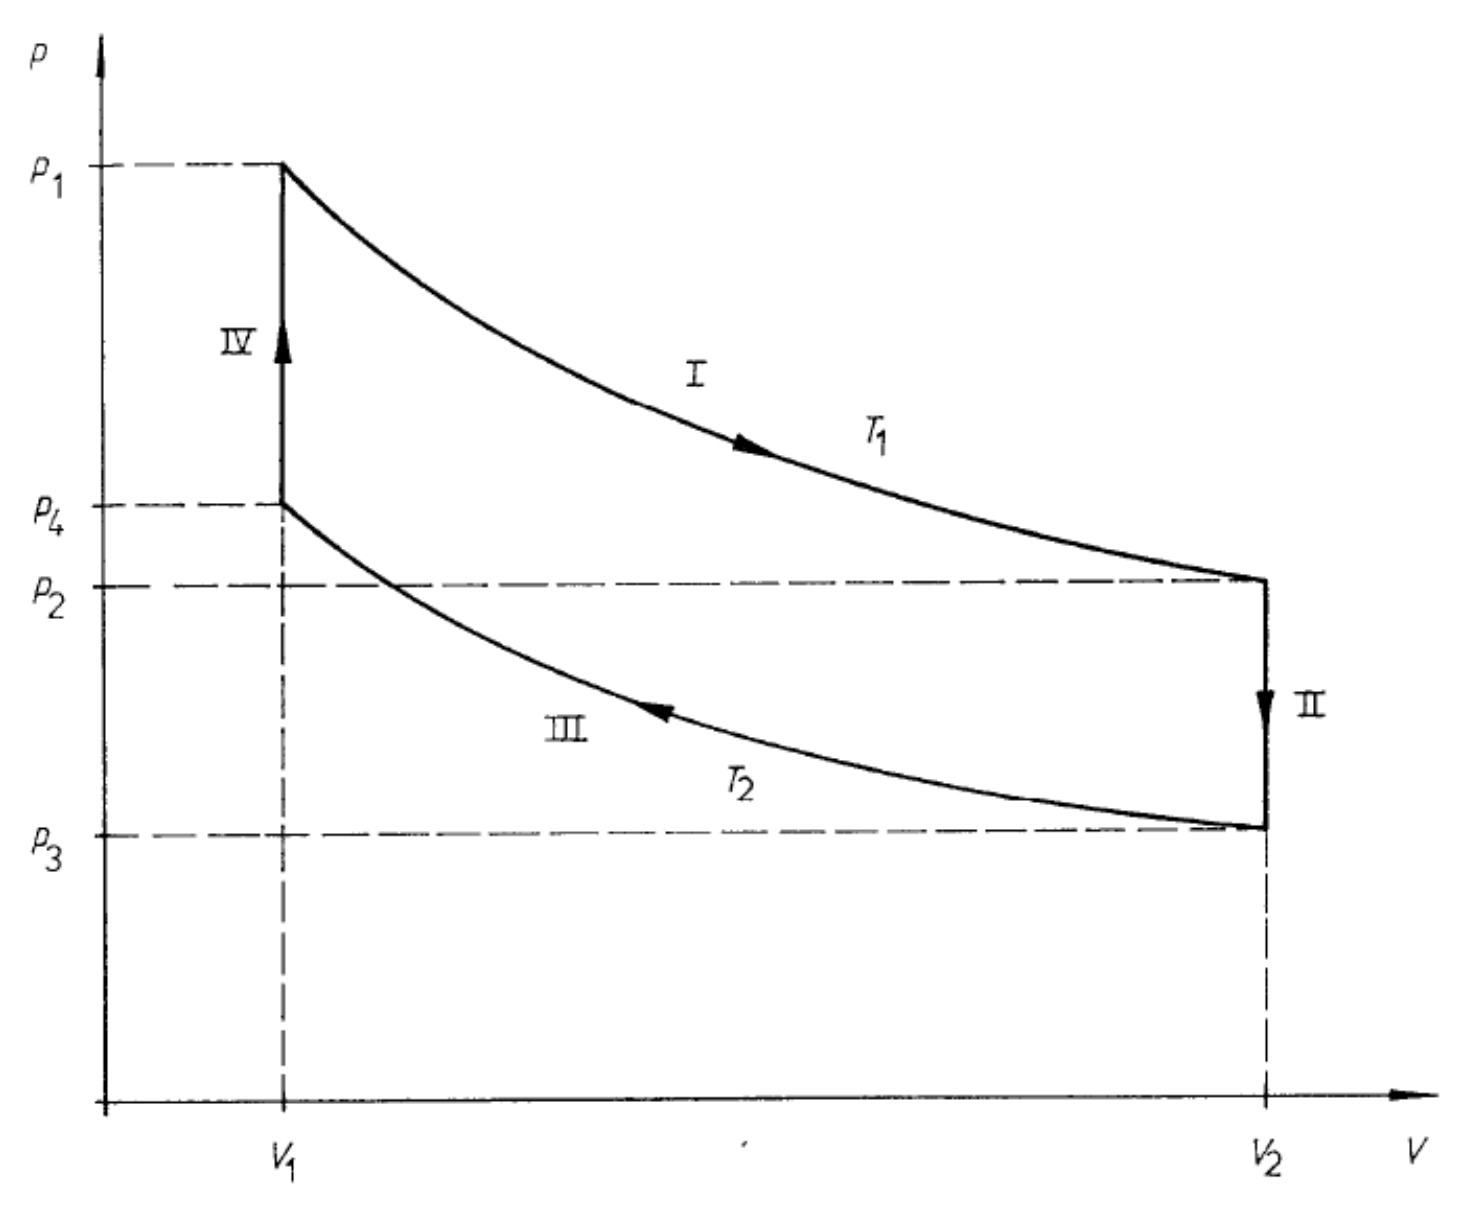
\includegraphics[width=0.5\textwidth]{../Figures/PV_diagram.png}
    \caption{PV diagram of Stirling's Engine}
    \label{fig:PV_diagram}
\end{figure}
\subsection{Derive expressions for the heat flow in (or out) and the work done by each step in the Stirling cycle}

The internal energy, heat and work done by the gas of a ideal gas follows 
the relationship,

\begin{equation}
    \Delta U = Q - W.
\end{equation}

From Figure \ref{fig:PV_diagram},

I: This is an isothermal expansion, so there is no change 
in internal energy,

\begin{equation}
    \Delta U = 0.
\end{equation}

Therefore, to find the heat flow of this isothermal process, we can 
exploit the fact that the heat absorbed by the expansion of the gas 
is equal to the work done by the gas,

\begin{equation}
    Q = W.
\end{equation}

The work done by the gas can be found using the formula,

\begin{equation}
    W = \int_{V_i}^{V_f} P dV.
\end{equation}

If we use the ideal gas law and substitute P with an equation 
involving V,

\begin{align}
    PV &= nRT \\
    P &= \frac{nrT}{V}.
\end{align}

We obtain

\begin{equation}
    W = \int_{V_i}^{V_f} \frac{nRT}{V} dV.
\end{equation}

Since temperature is constant in an isothermal process,

\begin{equation}
    W = nRT \int_{V_i}^{V_f}\frac{1}{V} dV.
\end{equation}

Completing the integral,

\begin{equation}
    W = nRT \log{\frac{V_f}{V_i}}.
\end{equation}

And so the heat absorbed by the gas as it expands is

\begin{equation}
    Q = nRT \log{\frac{V_f}{V_i}}.
\end{equation}

III: Since this is also an isothermal process it will follow 
the same process as in I, however the signage of the work done 
by the gas and the heat it absorbs changes. This is representative 
of the fact that now the gas is being compressed and so work is done 
on it and to ensure the temperature is constant, it must release heat.

II: This is an isochoric process and so the work done is 0.
This means that the heat transferred is equal to the internal energy 
change of the gas,

\begin{equation}
    Q = \Delta U.
\end{equation}

We can then use the formula,

\begin{equation}
    Q = n C_v \Delta T.
\end{equation}

In this specific process, II, there is a depressurisation meaning heat 
and energy are both released.

IV: This is a isochoric pressurisation meaning there is an inflow of heat 
and thus an increase in internal energy.

\subsection{Calculate the heat flow in each step}
We are given the following values for a monoatomic gas
undergoing the Stirling Cycle,

\begin{align}
    T_{upper} &= 400 \text{ K} \\
    T_{lower} &= 300 \text{ K} \\
    V_{max} &= 10\text{ m}^3 \\
    V_{min} &= 2\text{ m}^3.
\end{align}

Since it is a monoatomic gas, 
\begin{equation}
    C_V = \frac{3}{2}R.
\end{equation}

I: The heat absorbed is 

\begin{equation}
    Q = nRT \log{\frac{V_f}{V_i}}.
\end{equation}

Substituting in values,

\begin{align}
    Q &= n (8.314)(400)\log{\frac{10}{2}} \\
    &= 5352.0 \text{J per mole}
\end{align}

II: The heat released is 

\begin{equation}
    Q = n C_v \Delta T. 
\end{equation}

Substituting in values,

\begin{align}
    Q &= n (3/2)(8.314)(300 - 400) \\
    &= -1247.1 \: \text{J per mole}
\end{align}

III: The heat released is 

\begin{equation}
    Q = nRT \log{\frac{V_f}{V_i}}.
\end{equation}

Substituting in values,

\begin{align}
    Q &= n (8.314)(300)\log{\frac{2}{10}} \\
    &= -4014.3 \: \text{J per mole}
\end{align}

IV: The heat absorbed is 

\begin{equation}
    Q = n C_v \Delta T. 
\end{equation}

Substituting in values,

\begin{align}
    Q &= n (3/2)(8.314)(400 - 300) \\
    &= 4014.3 \: \text{J per mole}
\end{align}

\subsection{Calculate the work done by the gas in the cycle}
Aforementioned, work done is 0 in processes II and IV. The work 
done by the gas in I is simply equal to the heat absorbed whilst
the work done on the gas in III is equal to the heat released.

\subsection{Calculate the efficiency of the engine}
The efficiency of the engine is calculated by taking the quotient of 
the work done by the gas and the work done on the gas and the heat 
absorbed by the gas,

\begin{align}
    \text{Efficiency} &= \frac{\text{output}}{\text{input}} \\
    &= \frac{\text{work done by the gas}}{\text{work done on the gas} + \text{
    heat absorbed}} \\
    &= \frac{1247.1}{4014.3+1247.1} \\
    &= 23.7 \%.
\end{align}

\section{Experimental Prework}
\subsection{Explain how the torque meter works}
The torque from the Stirling engine will be countered by the torque created by 
the mass due to gravity, the counter torque increases as the mass is lifted 
up as the angle between the force of gravity and the radius from the centre 
of the torque meter increases. The two torques will be equal when the contraption 
stops and since the torque due to gravity is easily calculated, the scale can be 
used to indciate the torque due to the engine.

\section{Appendix}
\subsection{Raw Data}
% Table generated by Excel2LaTeX from sheet 'Final Mechanical Power'
\begin{table}[H]
    \centering
      \begin{tabular}{c|c|c|c|c|c|c}
      \multicolumn{1}{l}{$\tau$ (10$^{-3}$Nm$^{-1}$)} & \multicolumn{1}{l}{$T_h$ (K)} & \multicolumn{1}{l}{$T_c$ (K)} & \multicolumn{1}{l}{$\Delta T$ (K)} & \multicolumn{1}{l}{$f$ (s$^{-1}$)} & \multicolumn{1}{l}{$\omega$ rads$^{-1}$} & \multicolumn{1}{l}{$P$ (Js$^{-1}$)} \\
      \hline
      0     & 171.5 & 60.2  & 111.3 & 18.24 & 114.6053 & 0 \\
      3     & 164.5 & 58.6  & 105.9 & 17.77 & 111.6522 & 334.9566 \\
      4.5   & 203.2 & 65.6  & 137.6 & 16.03 & 100.7195 & 453.2376 \\
      9     & 190.5 & 63.6  & 126.9 & 13.15 & 82.62389 & 743.615 \\
      7     & 182.2 & 62.4  & 119.8 & 13.61 & 85.51415 & 598.5991 \\
      12    & 177.6 & 61    & 116.6 & 10.47 & 65.78495 & 789.4194 \\
      14.5  & 172.9 & 59.4  & 113.5 & 7.76  & 48.75752 & 706.984 \\
      15.5  & 175.8 & 58.4  & 117.4 & 7.05  & 44.29646 & 686.5951 \\
      16.5  & 186   & 55.7  & 130.3 & 6.29  & 39.52124 & 652.1004 \\
      17    & 192.9 & 54.7  & 138.2 & 4.77  & 29.97079 & 509.5035 \\
      18    & 220.7 & 54.1  & 166.6 & 7.28  & 45.74159 & 823.3486 \\
      19    & 242.5 & 57    & 185.5 & 5.61  & 35.24867 & 669.7247 \\
      19.5  & 253.4 & 58.6  & 194.8 & 5.66  & 35.56283 & 693.4752 \\
      20    & 249.1 & 58.2  & 190.9 & 4.7   & 29.53097 & 590.6194 \\
      \end{tabular}%
      \caption{Raw data obtained from mechanical power experiment}
    \label{tab:table1}%
  \end{table}%
% Table generated by Excel2LaTeX from sheet 'Electrical Power'
\begin{table}[H]
    \centering
      \begin{tabular}{c|c|c|c|c|c|c|c|c}
      \multicolumn{1}{l}{$R$ ($\Omega$)} & \multicolumn{1}{l}{$T_h$ (K)} & \multicolumn{1}{l}{$T_c$ (K)} & \multicolumn{1}{l}{$\Delta T$ (K)} & \multicolumn{1}{l}{$f$ (s$^{-1}$)} & \multicolumn{1}{l}{$\omega$ rads$^{-1}$} & \multicolumn{1}{l}{$\mathcal{E}$ (V)} & \multicolumn{1}{l}{$I$ (A)} & \multicolumn{1}{l}{$P$ (Js$^{-1}$)} \\
      \hline
      11111110 & 236.2 & 70.5  & 165.7 & 14.1  & 88.59291 & 6.5   & 0.0000013 & 8.45E-06 \\
      1111110 & 201.1 & 73.5  & 127.6 & 13.31 & 83.6292 & 6.56  & 0.0000065 & 4.26E-05 \\
      111110 & 187.4 & 73.1  & 114.3 & 12.5E+0 & 78.28849 & 6.4   & 0.0000581 & 0.000372 \\
      11110 & 186.4 & 73.1  & 113.3 & 12.53 & 78.72831 & 6     & 0.00055 & 0.0033 \\
      1110  & 199.5 & 75.1  & 124.4 & 12.44 & 78.16283 & 5.1   & 0.000463 & 0.002361 \\
      110   & 189.7 & 74.3  & 115.4 & 11.25 & 70.68583 & 3.6   & 0.0032 & 0.01152 \\
      70    & 186   & 72.5  & 113.5 & 10.27 & 64.52831 & 3.2   & 0.0046 & 0.01472 \\
      60    & 177   & 68.5  & 108.5 & 10.11 & 63.523 & 3     & 0.0047 & 0.0141 \\
      50    & 178   & 67.5  & 110.5 & 9.79  & 61.51238 & 2.8   & 0.0061 & 0.01708 \\
      40    & 198.3 & 69.1  & 129.2 & 9.18  & 57.67964 & 2.4   & 0.0066 & 0.01584 \\
      30    & 225.6 & 69.9  & 155.7 & 8.98  & 56.423 & 2.2   & 0.0084 & 0.01848 \\
      20    & 204   & 68.9  & 135.1 & 7.34  & 46.11858 & 1.6   & 0.0095 & 0.0152 \\
      10    & 210   & 69.3  & 140.7 & 6.16  & 38.70442 & 0.8   & 0.013 & 0.0104 \\
      8     & 200.5 & 66.7  & 133.8 & 6.42  & 40.33805 & 0.78  & 0.014 & 0.01092 \\
      6     & 203.4 & 65.8  & 137.6 & 5.79  & 36.37964 & 0.58  & 0.0155 & 0.00899 \\
      4     & 235.4 & 66    & 169.4 & 5.56  & 34.93451 & 0.4   & 0.018 & 0.0072 \\
      2     & 214.4 & 64.4  & 150   & 5.06  & 31.79292 & 0.2   & 0.0196 & 0.00392 \\
      700   & 205.8 & 67.3  & 138.5 & 12.21 & 76.71769 & 5.2   & 0.00049 & 0.002548 \\
      400   & 197.1 & 70.7  & 126.4 & 11.08 & 69.61769 & 4.4   & 0.00096 & 0.004224 \\
      600   & 190.7 & 70.3  & 120.4 & 11.83 & 74.33008 & 4.7   & 0.00063 & 0.002961 \\
      500   & 198.5 & 71.5  & 127   & 11.79 & 74.07875 & 4.5   & 0.00099 & 0.004455 \\
      \end{tabular}%
      \caption{Raw data obtained from electrical power experiment}
    \label{tab:table2}%
  \end{table}%

\subsection{Code snippets}
\begin{python}
#Theoretical Model
def curve(x,a,b,c):
    return a*x**2 + b*x + c
def curve2(t,T_0,T_h,T_c,k):
    return T_0 + (T_h - T_c)*np.exp(-k*t)
\end{python}

\begin{python}
#Error for Mech Power
t1std = np.std(df1['T1'])
t2std = np.std(df1['T2'])

t1mean = np.mean(df1['T1'])
t2mean = np.mean(df1['T2'])

t1err = t1std/t1mean 
t2err = t2std/t2mean

print(t1err,t2err)

xerr1 = np.sqrt(t1err**2+t2err**2)
print(xerr1)

yerr1 = np.mean([0.5/x for x in df1['Torque Meter'] if x > 0])
print(yerr1)
\end{python}

\begin{python}
#Error for Elec Power
t1std = np.std(df2['T1'])
t2std = np.std(df2['T2'])

t1mean = np.mean(df2['T1'])
t2mean = np.mean(df2['T2'])

t1err = t1std/t1mean 
t2err = t2std/t2mean

print(t1err,t2err)

xerr2 = np.sqrt(t1err**2+t2err**2)
print(xerr2)

def digit(V):
    if V == 0 or not isinstance(V,(int,float)) or math.isnan(V):
        return 0
    number = '0.'
    for i in range(1,len(str(V))-2):
        number += '0'
        i += 1
    return float(number + str(abs(V))[-1])

verrlst = [0.009 * V + 2*digit(V) if isinstance(V,(int,float)) and not math.isnan(V) else None for V in df2s['Voltage (V)']]
aerrlst = [0.018 * A + 2*digit(A) if isinstance(A,(int,float)) and not math.isnan(A) else None for A in df2s['Current (A)']]

def average(lst):
    clean_lst = [x for x in lst if x is not None]
    return sum(clean_lst)/len(clean_lst) if clean_lst else None

verr = average(verrlst)
aerr = average(aerrlst)

yerr2 = np.sqrt(verr**2+aerr**2+0.01**2)
print(yerr2)
\end{python}

\section{Lab Book Pages}
\begin{figure}[H]
    \centering
    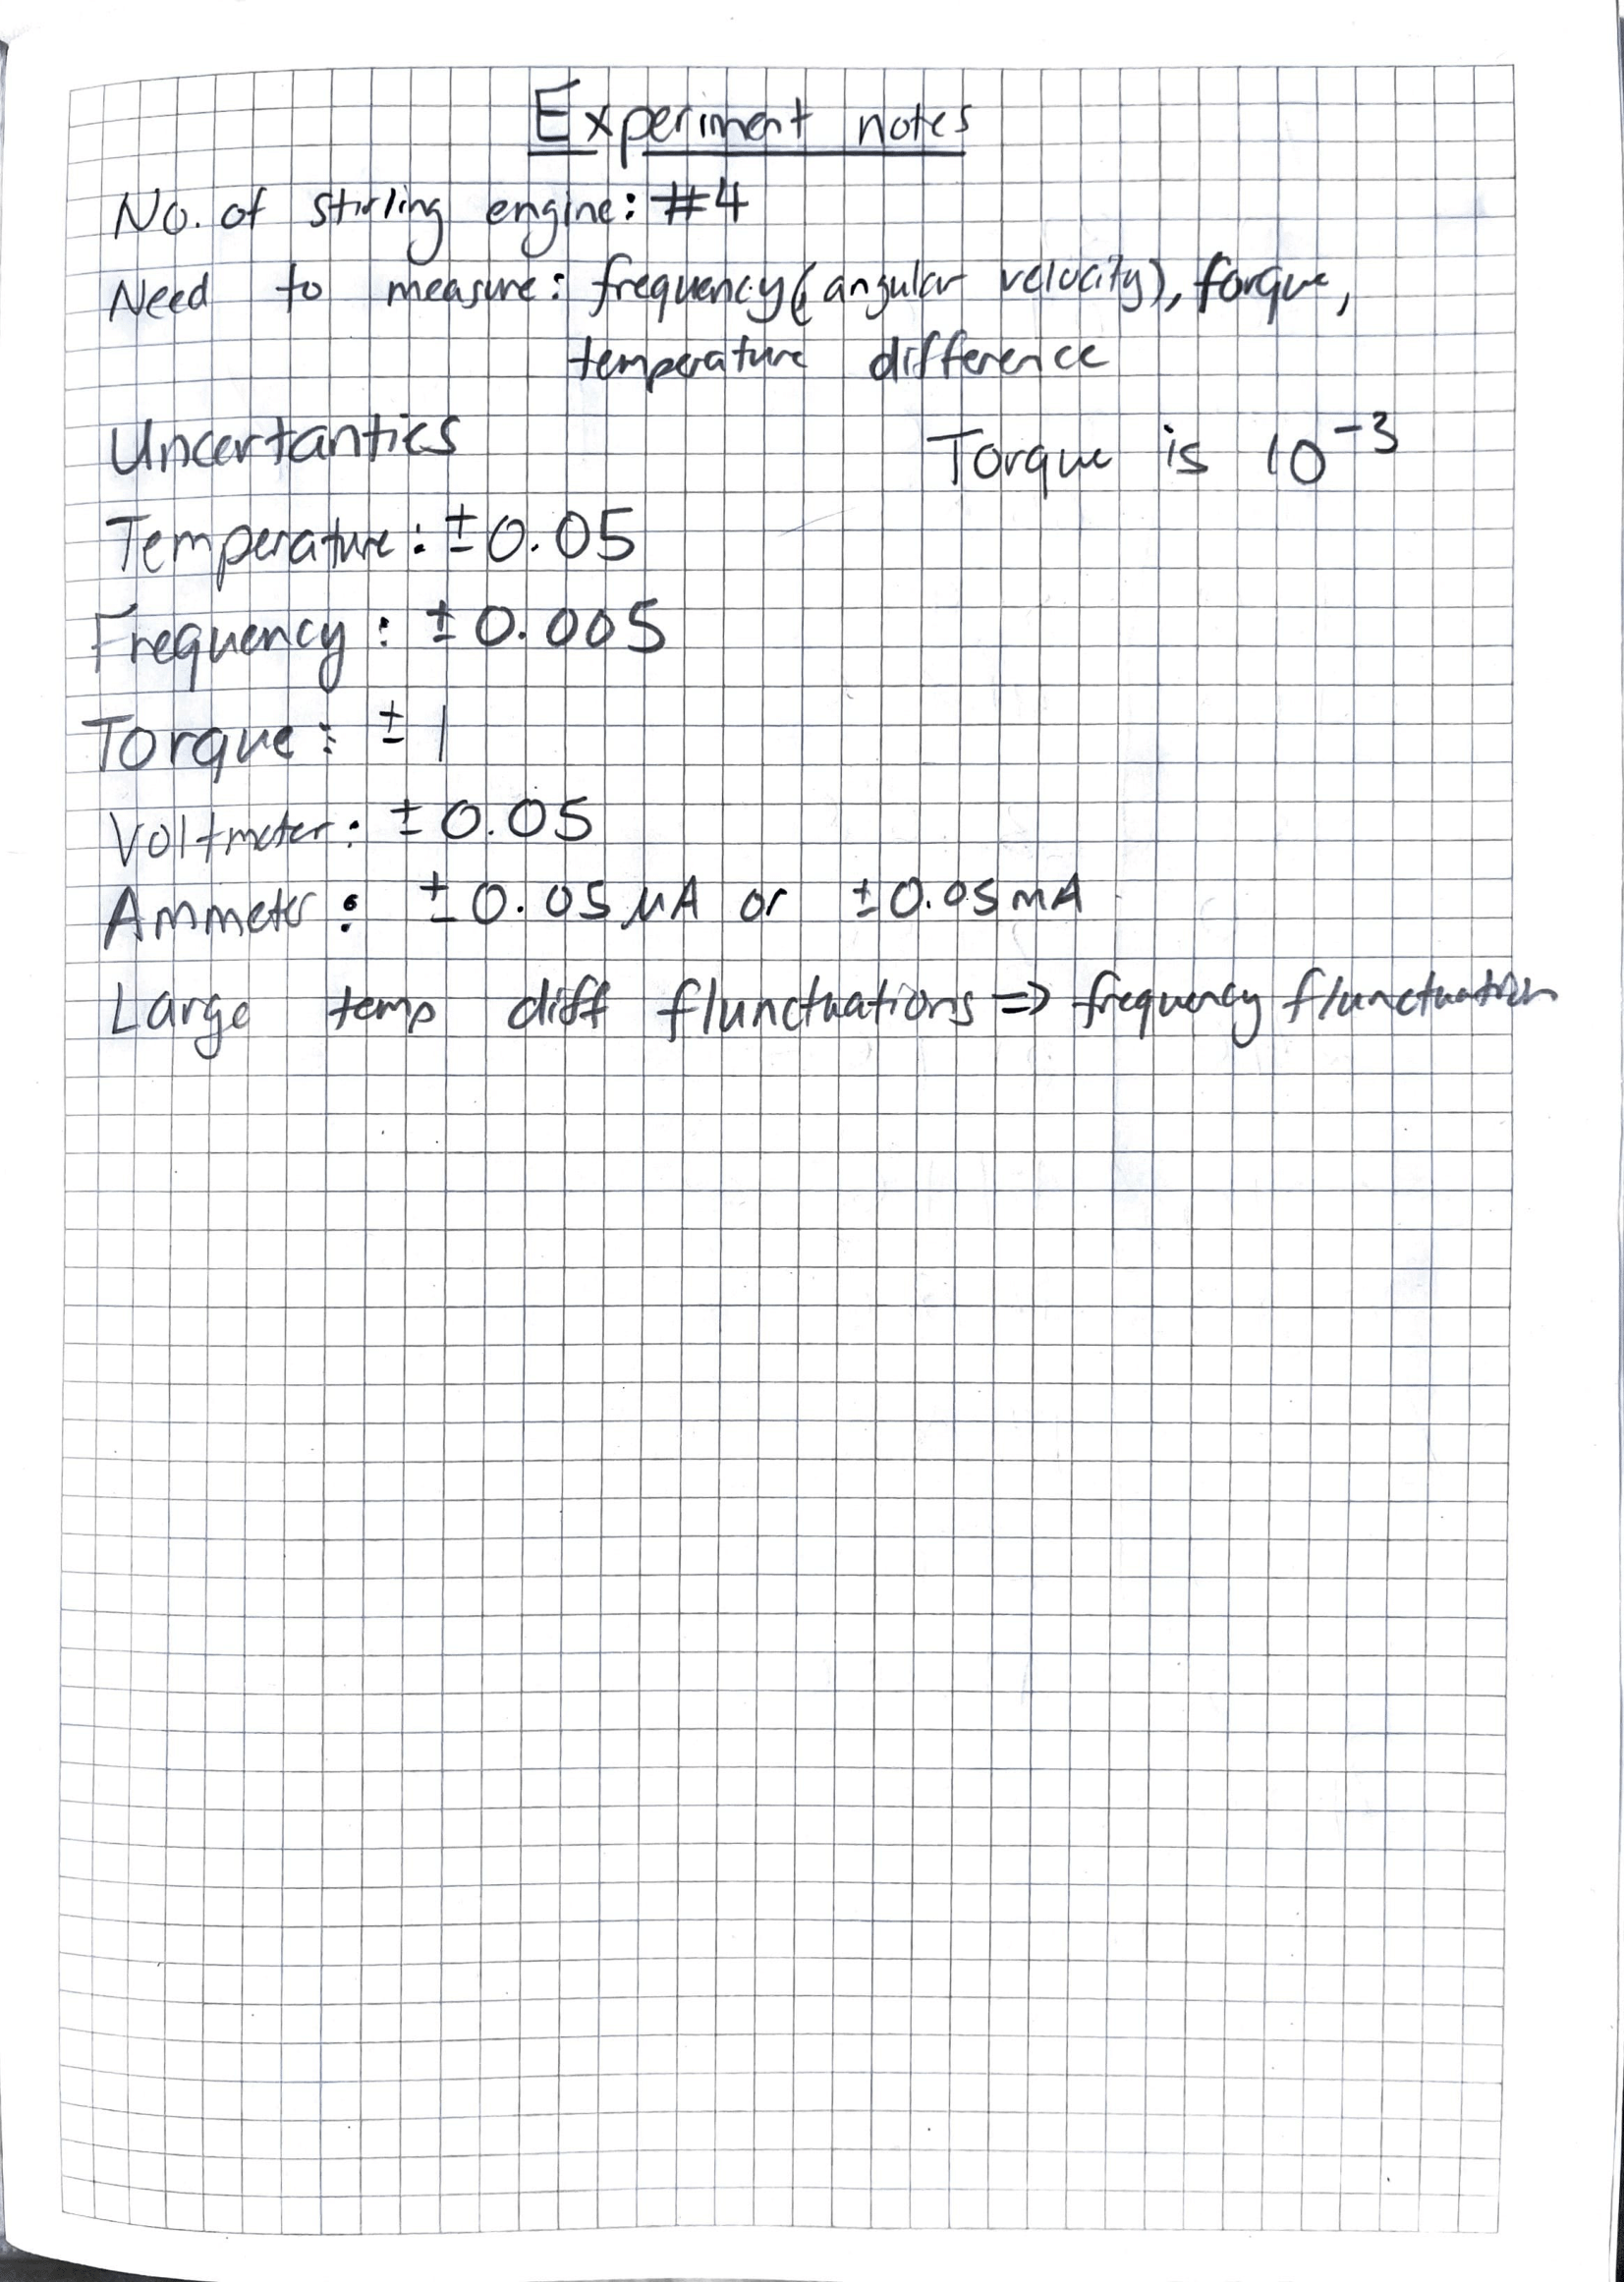
\includegraphics[width=0.7\textwidth]{../Figures/Labbook1.png}
\end{figure}
\begin{figure}[H]
    \centering
    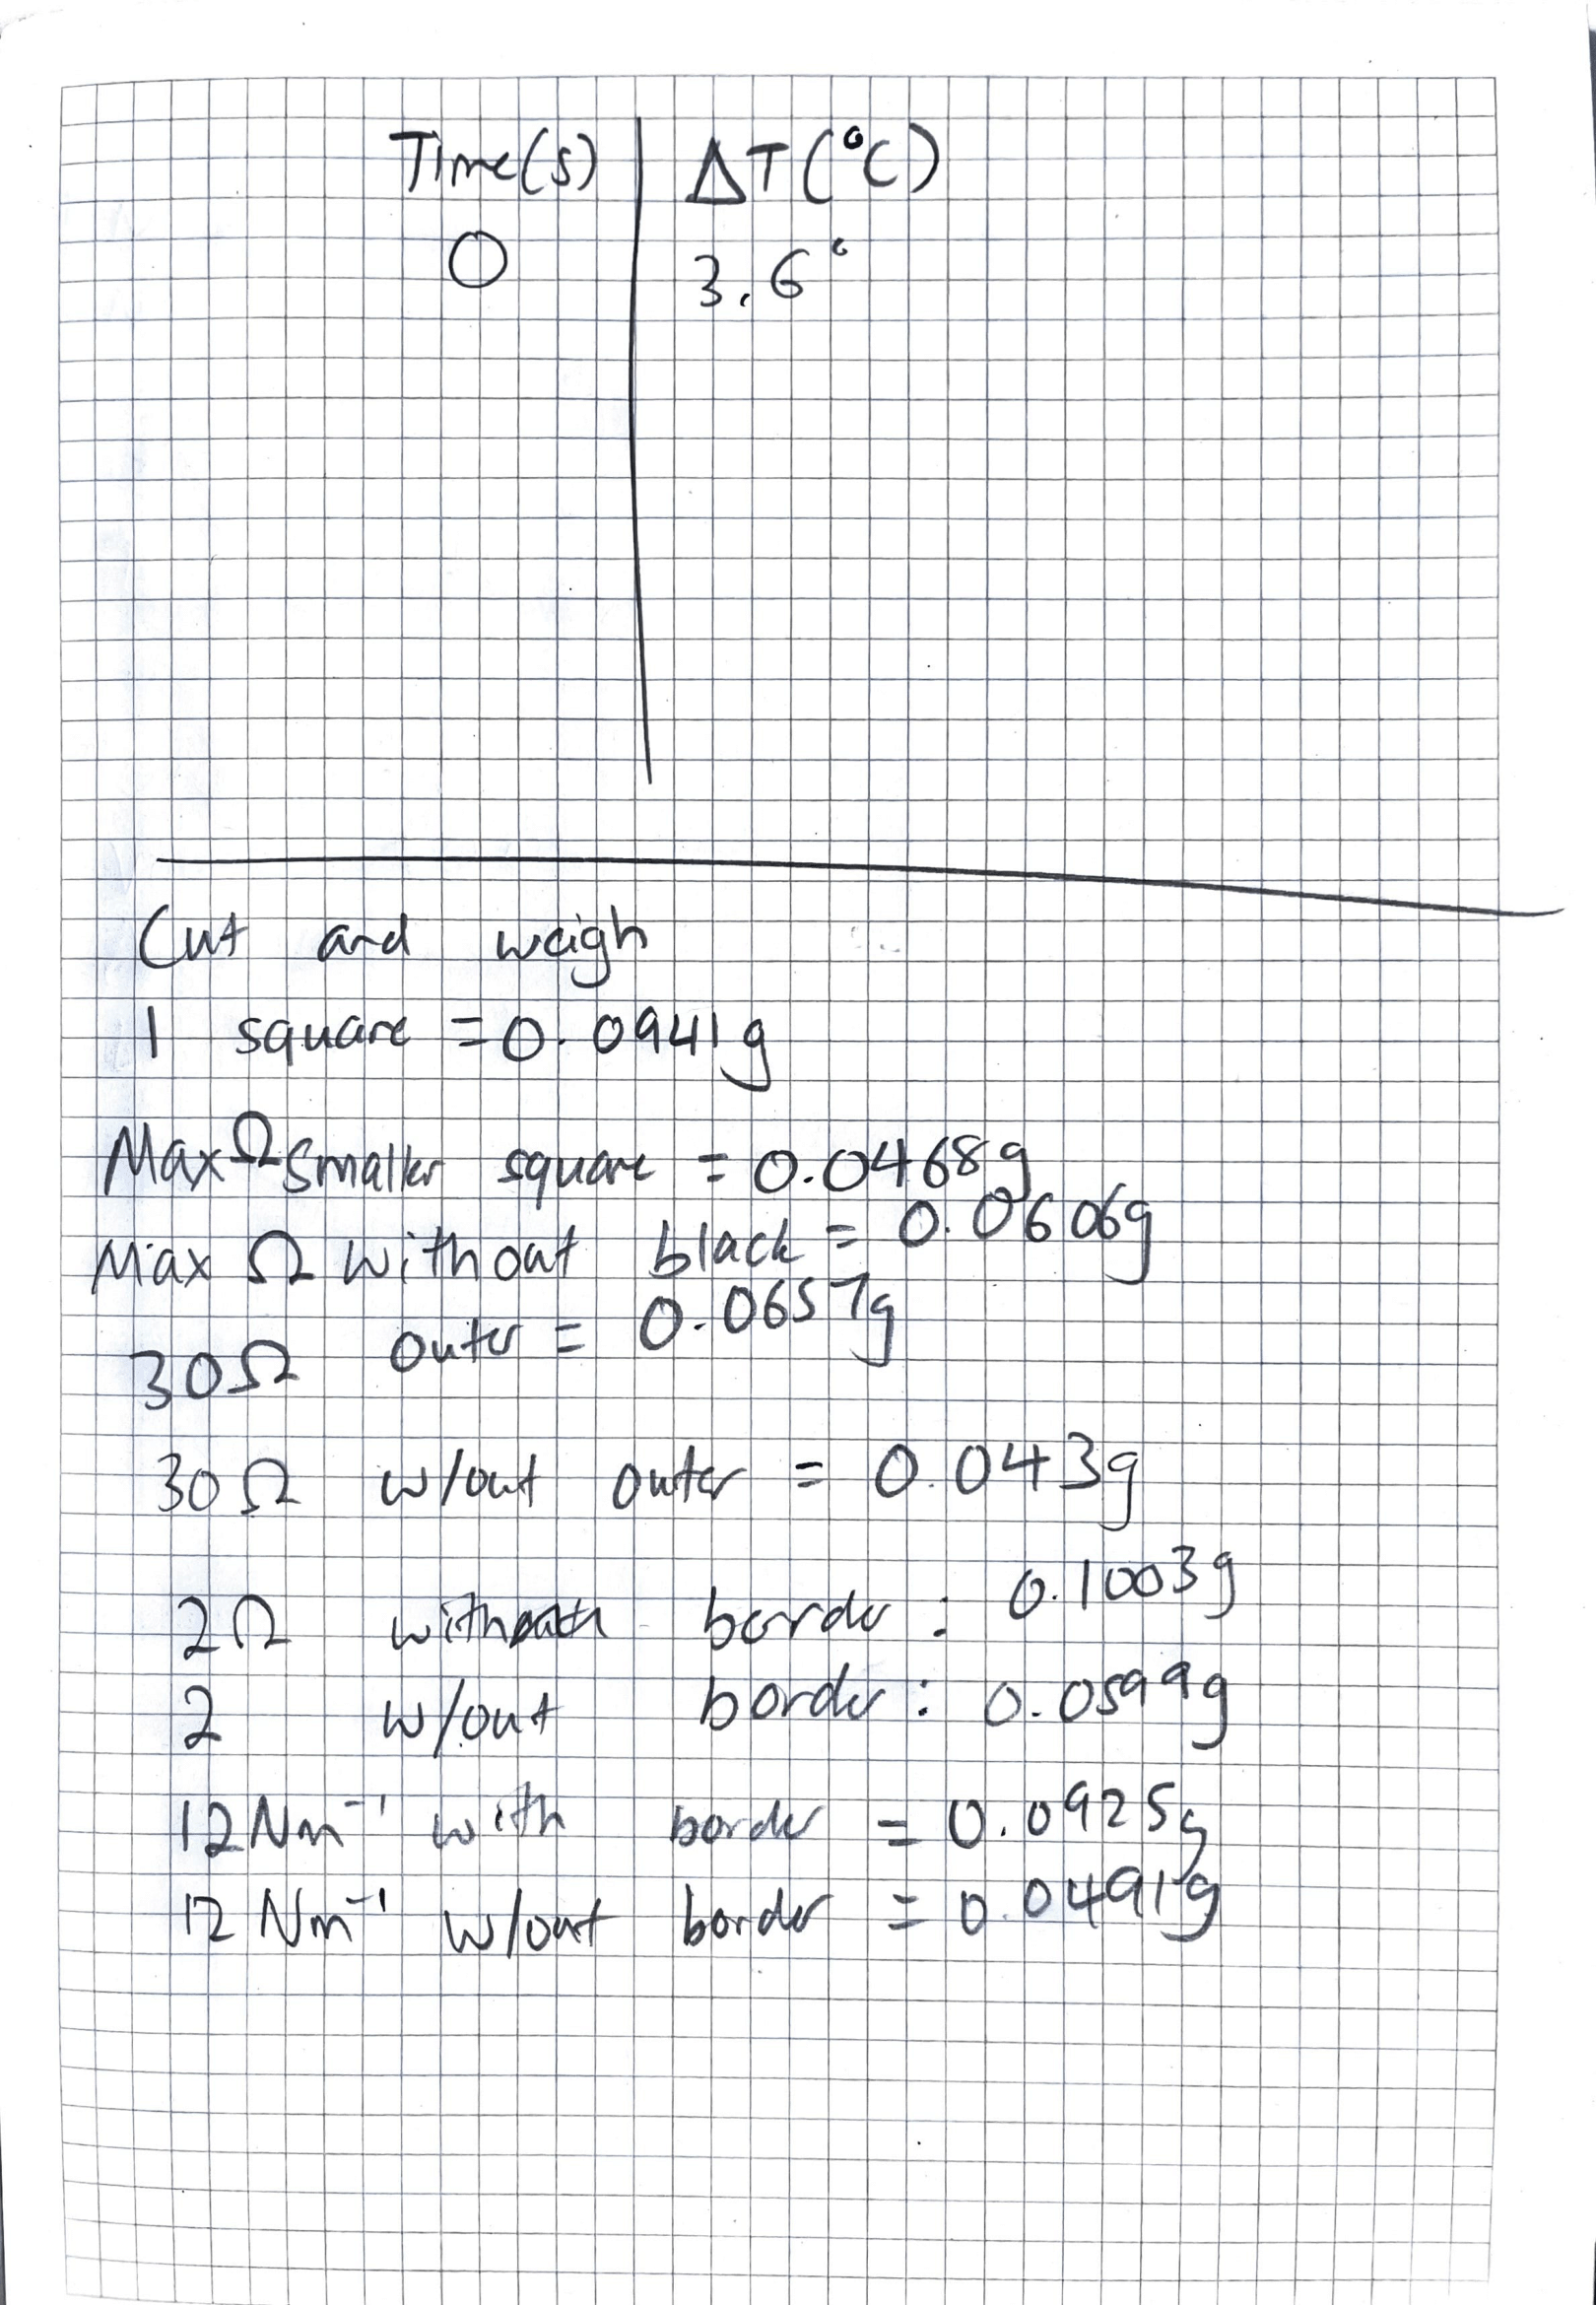
\includegraphics[width=0.7\textwidth]{../Figures/Labbook2.png}
\end{figure}
\begin{figure}[H]
    \centering
    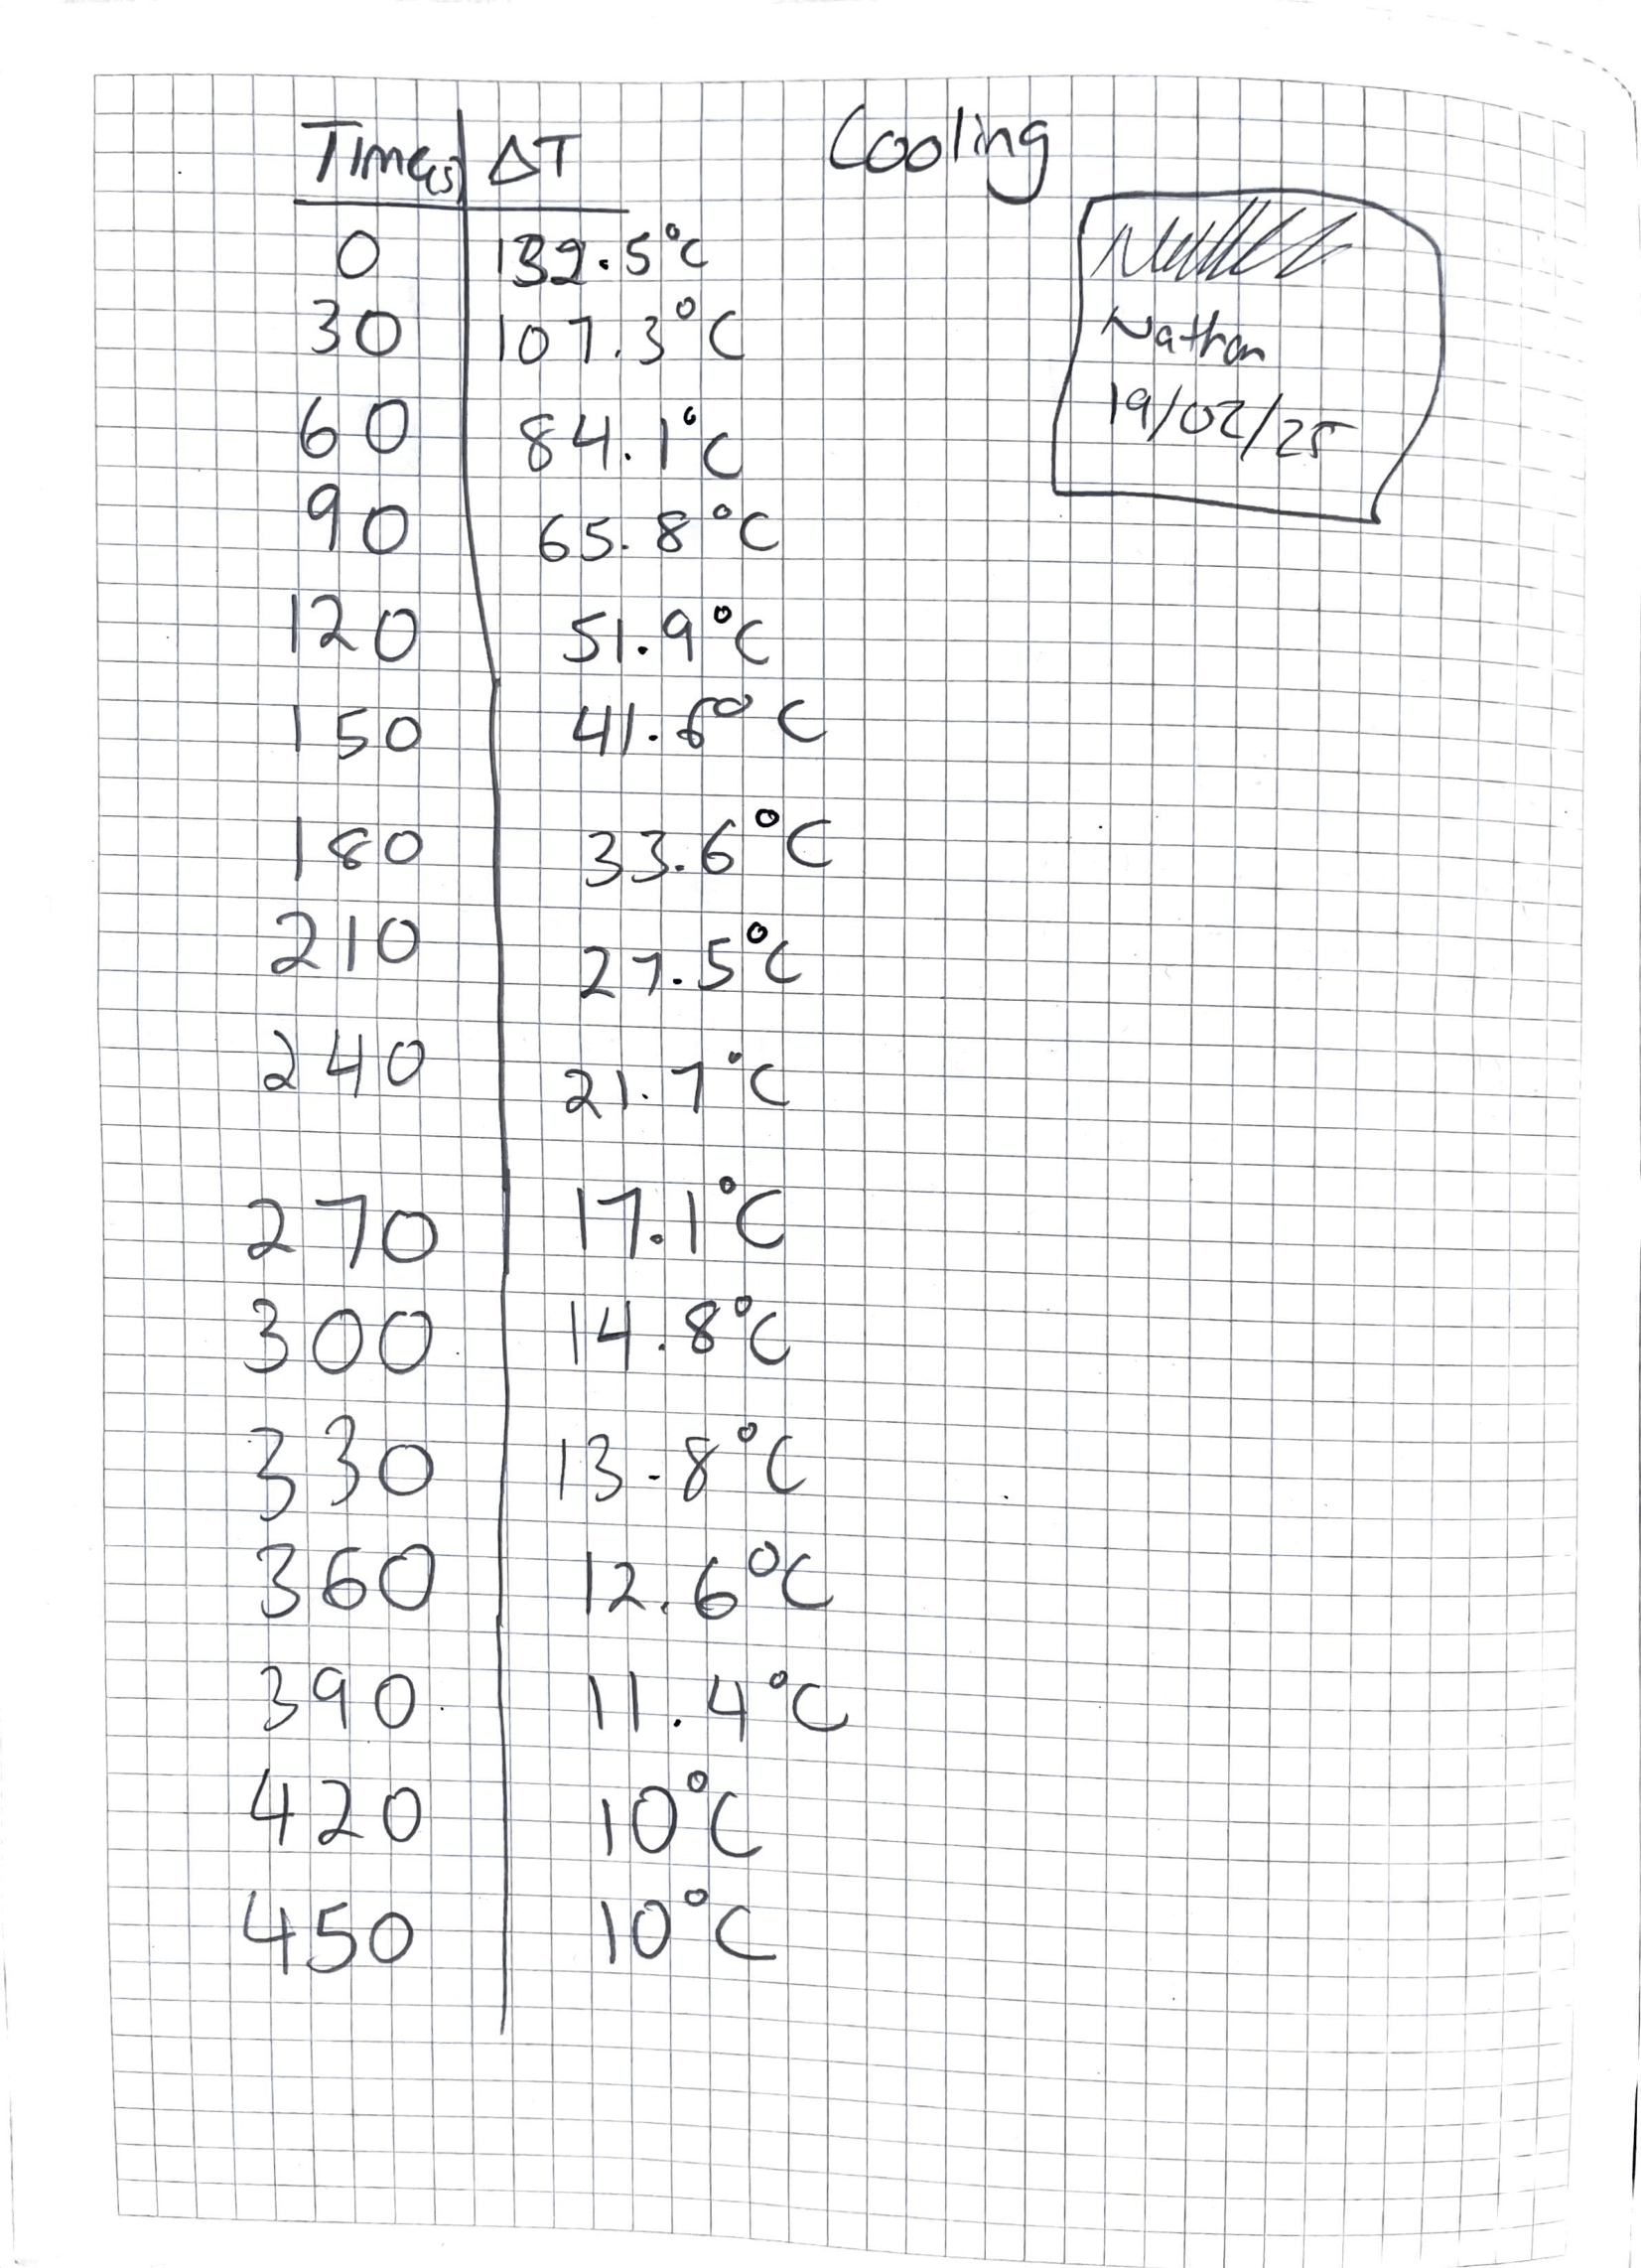
\includegraphics[width=0.7\textwidth]{../Figures/Labbook3.png}
\end{figure}

\end{document}